\documentclass[11pt,tikz,border=3pt]{standalone}

\usepackage[T1]{fontenc}
\usepackage{lmodern}
\usepackage{amsmath}
\usetikzlibrary{arrows.meta,calc,decorations.pathreplacing}

\definecolor{ink}{RGB}{47,52,57}
\definecolor{softgrey}{RGB}{235,237,239}
\definecolor{midgrey}{RGB}{151,157,163}
\definecolor{physicalfill}{RGB}{218,234,246}
\definecolor{physicalblue}{RGB}{0,114,178}
\definecolor{oddorange}{RGB}{213,94,0}
\definecolor{panelborder}{RGB}{190,195,200}

\begin{document}
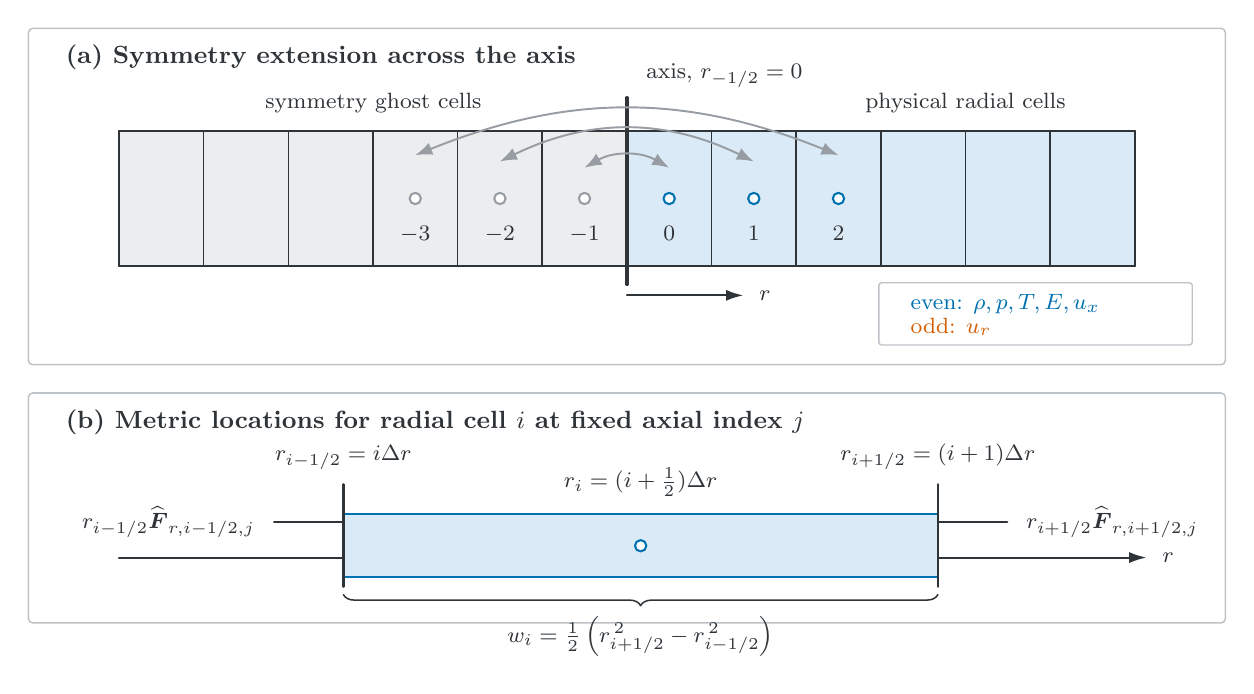
\begin{tikzpicture}[
    x=1cm,
    y=1cm,
    font=\rmfamily\footnotesize,
    line cap=round,
    line join=round,
    >=Latex,
    panel/.style={
      draw=panelborder,
      line width=0.55pt,
      rounded corners=1.5pt
    },
    paneltitle/.style={
      anchor=west,
      font=\rmfamily\small\bfseries,
      text=ink
    },
    label/.style={
      text=ink
    },
    face/.style={
      draw=ink,
      line width=0.55pt
    },
    centre/.style={
      circle,
      draw=physicalblue,
      fill=white,
      line width=0.75pt,
      inner sep=1.45pt
    },
    ghostcentre/.style={
      circle,
      draw=midgrey,
      fill=white,
      line width=0.75pt,
      inner sep=1.45pt
    }
]

% Panel (a): parity extension at the cylindrical axis.
\draw[panel] (0,3.28) rectangle (15.2,7.55);
\node[paneltitle] at (0.35,7.18)
  {(a) Symmetry extension across the axis};

\fill[softgrey] (1.15,4.53) rectangle (7.60,6.25);
\fill[physicalfill] (7.60,4.53) rectangle (14.05,6.25);

\foreach \x in {1.15,2.225,3.30,4.375,5.45,6.525,7.60,
                 8.675,9.75,10.825,11.90,12.975,14.05} {
  \draw[face] (\x,4.53) -- (\x,6.25);
}
\draw[draw=ink,line width=0.75pt] (1.15,4.53) rectangle (14.05,6.25);
\draw[draw=ink,line width=1.25pt] (7.60,4.30) -- (7.60,6.67);

\node[label,anchor=south] at (4.38,6.36) {symmetry ghost cells};
\node[label,anchor=south] at (11.90,6.36) {physical radial cells};
\node[label,anchor=south west] at (7.72,6.67)
  {axis, \(r_{-1/2}=0\)};

% Radial coordinate arrow.  The axial coordinate is fixed in this indexing
% sketch, so no second arrow is drawn through the cell-index labels.
\draw[-{Latex[length=2.2mm,width=1.4mm]},draw=ink,line width=0.75pt]
  (7.60,4.16) -- (9.08,4.16);
\node[label,anchor=west] at (9.16,4.16) {\(r\)};

% Three mirrored pairs are enough to define the indexing without crowding.
\foreach \x/\idx in {
  4.9125/{-3},
  5.9875/{-2},
  7.0625/{-1}
} {
  \node[ghostcentre] at (\x,5.39) {};
  \node[label,anchor=north] at (\x,5.16) {\(\idx\)};
}
\foreach \x/\idx in {
  8.1375/{0},
  9.2125/{1},
  10.2875/{2}
} {
  \node[centre] at (\x,5.39) {};
  \node[label,anchor=north] at (\x,5.16) {\(\idx\)};
}

% Mirrored-index guides.
\draw[draw=midgrey,line width=0.70pt,<->]
  (7.0625,5.78) to[bend left=30] (8.1375,5.78);
\draw[draw=midgrey,line width=0.70pt,<->]
  (5.9875,5.86) to[bend left=26] (9.2125,5.86);
\draw[draw=midgrey,line width=0.70pt,<->]
  (4.9125,5.94) to[bend left=22] (10.2875,5.94);

% Parity key.
\draw[draw=panelborder,fill=white,line width=0.50pt,rounded corners=1pt]
  (10.80,3.53) rectangle (14.78,4.32);
\node[text=physicalblue,anchor=west] at (11.08,4.05)
  {even: \(\rho,p,T,E,u_x\)};
\node[text=oddorange,anchor=west] at (11.08,3.76)
  {odd: \(u_r\)};

% Panel (b): locations and weights for a generic physical radial cell.
\draw[panel] (0,0) rectangle (15.2,2.92);
\node[paneltitle] at (0.35,2.55)
  {(b) Metric locations for radial cell \(i\) at fixed axial index \(j\)};

\draw[-{Latex[length=2.2mm,width=1.4mm]},draw=ink,line width=0.75pt]
  (1.15,0.83) -- (14.20,0.83);
\node[label,anchor=west] at (14.28,0.83) {\(r\)};

\draw[draw=physicalblue,fill=physicalfill,line width=0.85pt]
  (4.00,0.58) rectangle (11.55,1.38);
\draw[draw=ink,line width=0.85pt] (4.00,0.46) -- (4.00,1.76);
\draw[draw=ink,line width=0.85pt] (11.55,0.46) -- (11.55,1.76);
\node[centre] at (7.775,0.98) {};

\node[label,anchor=south] at (4.00,1.82)
  {\(r_{i-1/2}=i\Delta r\)};
\node[label,anchor=south] at (7.775,1.48)
  {\(r_i=(i+\tfrac{1}{2})\Delta r\)};
\node[label,anchor=south] at (11.55,1.82)
  {\(r_{i+1/2}=(i+1)\Delta r\)};

\draw[draw=ink,line width=0.85pt]
  (4.00,1.28) -- (3.12,1.28);
\draw[draw=ink,line width=0.85pt]
  (11.55,1.28) -- (12.43,1.28);
\node[label,anchor=east] at (3.00,1.28)
  {\(r_{i-1/2}\widehat{\boldsymbol F}_{r,i-1/2,j}\)};
\node[label,anchor=west] at (12.55,1.28)
  {\(r_{i+1/2}\widehat{\boldsymbol F}_{r,i+1/2,j}\)};

\draw[
  decorate,
  decoration={brace,mirror,amplitude=4pt},
  draw=ink,
  line width=0.55pt
] (4.00,0.36) -- (11.55,0.36);
\node[label,anchor=north] at (7.775,0.20)
  {\(\displaystyle
    w_i=\tfrac{1}{2}
    \left(r_{i+1/2}^{\,2}-r_{i-1/2}^{\,2}\right)\)};

\end{tikzpicture}
\end{document}
